本章将介绍模型所使用的对比学习范式,并讨论推荐系统的存在的公平性与数据偏见。之后,本章将提出 TAGCL 的设计架构,讨论了该框架是如何使用多任务学习进行训练并调优。

\section{对比学习}
本小节将简要回顾对比学习,并讨论其最为重要的 InfoNCE 损失函数是如何从 NCE 损失函数发展而来。
\subsection{对比学习回顾}
对比学习(Contrastive Learning, CL)是自监督学习(Self-Supervised Learning,SSL)中的一种方法,其旨在利用未标记的大量数据来学习知识。图~\ref{tag:dollar}~展示了对比学习的经典案例\footnote{摘录自:https://aeon.co/essays/your-brain-does-not-process-information-and-it-is-not-a-computer},以便更好地理解这种学习方法。具体而言,图~\ref{fig:rough}~是人工绘制的一张1美元纸币的图像,而图~\ref{fig:detailed}~则是一张真实的1美元纸币的图像。如果对这两张图像进行标注,我们会认为它们都属于 “1美元” 这个类别。然而,如果在像素级别上进行比较,可以明显看到两张图像存在巨大的差异:图~\ref{fig:rough}~不仅丢失了许多边缘细节,而且人脸朝向和 “one dollar” 的位置等关键信息也完全不同。

在使用监督学习模型的情况下,模型会将这两个数据样本视为独立的样本,并将它们分别输入模型进行学习。然而,由于这两个数据样本属于相同的标签,模型容易感到困惑,使得模型优化损失函数变得不稳定。相比之下,对比学习将这两张图像视为一对样本,并要求模型最大化它们在投影空间中的互信息,以便促进模型捕捉两张图像的相似性。

\begin{figure}[!h]
    \centering
    \begin{subfigure}{0.49\linewidth}
        \centering
        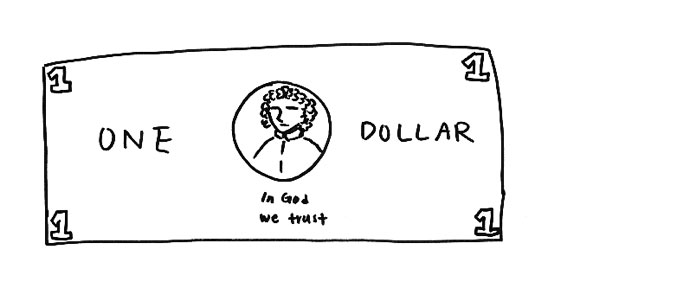
\includegraphics[width=.88\linewidth]{figure/Inline-rough.jpg}
        \caption{靠记忆复原的一美元}
        \label{fig:rough}
    \end{subfigure}
    \begin{subfigure}{0.49\linewidth}
        \centering
        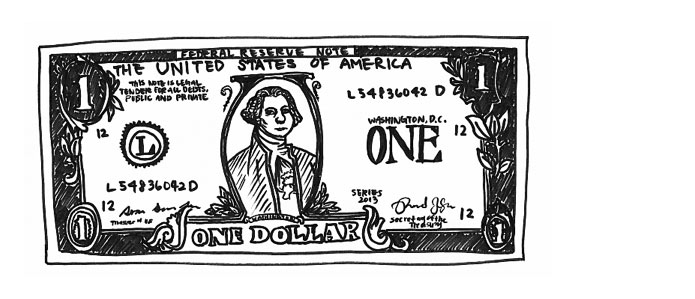
\includegraphics[width=.88\linewidth]{figure/Inline-Detailed.jpg}
        \caption{拥有细节的一美元}
        \label{fig:detailed}
    \end{subfigure}
    \caption{一个经典的对比学习例子}
    \label{tag:dollar}
\end{figure}

对比学习通过采用数据增强方法来构造相似和不相似的数据,并要求模型能够区分这些数据,从而使得相似的数据在投影空间中更为接近,而不相似的数据在投影空间中距离较远。对于对比学习模型来说,除了必备的编码器模块(Encoder)之外,还需要数据增广模块来生成单条数据样本的不同视图,以及对比学习模块,该模块通常采用噪声对比估计(Noise Contrastive Estimation,NCE)作为目标函数,以最大化同一数据样本不同视图之间的一致性以及不同样本的视图之间的差异性。本小节将以语言模型为例,深入介绍噪声对比估计,为后续内容提供理论基础。


\subsection{噪声对比估计}
本小节将以语言模型为例,深入介绍噪声对比估计。在语言模型中,给定一个序列,模型的目标是预测该序列的下一个单词。由于该模型在对参数进行极大似然估计时,需要存在较高的计算复杂度,因此噪声对比估计最初为了简化计算而被提出。
\subsubsection{语言模型}
语言模型(language model)是一种用于计算句子或文本的概率模型。它假设一门语言的所有可能的单词组合服从一定的概率分布。若将句子 $s$ 看成是单词 $w$ 的序列 $s = \{w_1,\cdots, w_m\}$,那么语言模型就是构建一个参数为这些单词的概率模型预测句子成立的概率。同时,可以中间任意一个单词 $w_i$ 以外其余的单词视为第 $i$ 个单词的上下文 $c_i$。那么,这个语言模型以链式法则展开后,也可以以条件概率的形式表示:
\begin{equation}
    \begin{aligned}
        p(w_1,w_2,\cdots, w_m) &= p(w_1) \times p(w_2 | w_1) \times p(w_3 | w_1, w_2) \times \cdots \times p(w_m | w_1, \cdots, w_m) \\ 
        & = \prod_{i=1}^{m} p(w_i | w_1, \cdots, w_{i-1}, w_{i+1}, \cdots, w_m) \\
        & = \prod_{i=1}^{m} p(w_i | c_i), \label{for:languagemodel1}
    \end{aligned}
\end{equation}
由上式可知,语言模型是条件概率 $p(w|c)$ 的集合。然而,直接计算每个单词 $w$ 在整体语料库中的条件概率需要很大计算量。因此,在真实世界运用的统计学语言模型通常会引入马尔可夫假设,即“一个词出现的概率只取决于它之前有限的 $n$ 个词有关”,这便是 n-gram 模型,它将公式~\ref{for:languagemodel1} 简化为:
\begin{gather}
    p(w_1,w_2,\cdots, w_m) = \prod_{i=1}^{m} p(w_i | w_{i-n+1},\cdots,w_{i-1})
\end{gather}

在建模统计语言模型时,利用极大似然估计,根据公式~\ref{for:languagemodel1},可以得到其似然函数的对数形式:
\begin{gather}
    \mathcal{L}_{MLE} = \sum_{w_i \in s} logp_{\theta}(w_i | c_i)
\end{gather}
这样,当最大化这个似然函数 $\mathcal{L}_{MLE}$ 时,实际上就是将 $p(w|c)$ 视为 $w$ 和 $c$ 的函数,$\theta$ 为待定的模型参数:
\begin{gather}
    p_{\theta}(w|c) = F(w,c; \theta)
\end{gather}
当模型通过数据训练获得到最优参数 $\theta^*$ 时,函数 $F$ 将会被确定,那么任意的 $p(w|c)$ 都快可以使用这个模型 $F(w,c; \theta^*)$计算得出。

由于神经网络能够拟合任何函数,因此被引入到统计语言模型中。Bengio 等人\cite{bengio_neural_2003}提出了神经概率语言模型(Neural Probabilistic Language Model,NPLM)。其可以在包含任意大小的上下文中建模单词 $w$ 出现的概率。具体而言,它将语言模型视为一个多分类问题。若将单词库记为 $V = \{v_1, v_2, \cdots, v_|V|\}$ ,将$(w,c)$作为一对训练样本,在通过神经网络和 SoftMax 函数归一化后,可以输出一个向量 $\hat{y} = [\hat{y}_{i,1},\hat{y}_{i,2},\cdots,\hat{y}_{i,|V|}]$,其中每一维 $\hat{y}_{i,j}$ 表示当上下文为 $c_i$ 时,第 $i$ 个单词为单词库中第 $j$ 个单词 $v_j$ 的概率。训练时会迫使模型将最后单词库中概率最大的单词作为训练样本对中的 $w_i$。这样,通过一定的训练后,给神经网络一个上下文 $c_i'$,神经网络就可以端到端的预测下一个单词 $w_i'$。

假设输入到 SoftMax 函数前的结果为 $s_{theta}(w,c)$。实际上该输出可以表示单词 $w$ 在这个上下文 $c$ 中的匹配程度。那么单词 $w$ 出现的条件概率可以表示为:
\begin{equation}
    \begin{aligned}
        p_{\theta}(w|c) & = \frac{exp(s_{\theta})(w,c)}{\sum_{w' \in V} exp(s_{\theta})(w,c)} \\
        & = \frac{u_{\theta}(w,c)}{Z(c)} \label{for:nce2}
    \end{aligned}
\end{equation}
其中,$u_{\theta}(w,c) = exp(s_{\theta})(w,c)$ 表示得到单词 $w$ 的概率。令 $Z(c) = \sum_{w' \in V} exp(s_{\theta})(w,c)$ 表示当前单词库内所有单词的概率累和。由于单词库的数量一般十分巨大,因此计算 $Z(c)$ 是非常昂贵、耗时的一件事。在语言模型引入噪声对比估计则为了解决这个问题。

\subsubsection{NCE 损失函数}
噪声对比估计的核心思想是通过学习数据分布样本和噪声样本之间的区别\cite{mnih_fast_2012},以此发现数据中的一些特性。具体而言,噪声对比估计将问题从多分类问题转化为二分类问题。模型只需要可以区分数据样本和噪声样本就可以学习到最优参数 $\theta^*$。假设特定上下文 $c$ 的数据分布为 $\tilde{p}(w|c)$,从该概率取出的样本为正样本,记类别为 $D = 1$,而另一个与 $c$ 无关的噪声分布为 $q(w)$,从该概率取出的样本为负样本,记类别为 $D = 0$。设从中取出 $k_d$ 个正样本和 $k_n$ 个负样本,再将这些正负样本混合成一个分布 $p(w|c)$。可以分别得到以下概率:
\begin{equation}
    \begin{aligned}
        p(D = 1) = \frac{k_d}{k_d + k_n} \\
        p(D = 0) = \frac{k_n}{k_d + k_n} \\
        p(w|D=1,c) = \tilde{p}(w|c) \\
        p(w|D=0,c) = q(w)
    \end{aligned}
\end{equation}
根据这些概率表达式,且记负样本和正样本之间的比例$k_n/k_d = k$,可以计算后验概率:
\begin{equation}
    \begin{aligned}
        p(D=0|w,c) = \frac{k \times q(w)}{\tilde{p}(w|c) + k \times q(w)} \\
        p(D=1|w,c) = \frac{\tilde{p}(w|c)}{\tilde{p}(w|c) + k \times q(w)}
    \end{aligned}
\end{equation}
根据噪声对比估计的假设,将 $Z(c)$ 作为一个参数 $z_c$ 进行估计,由公式~\ref{for:nce2}~可得:
\begin{equation}
    \begin{aligned}
        p_{\theta}(D=0|w,c) = \frac{k \times q(w)}{u_{\theta}(w,c) + k \times q(w)} \\
        p_{\theta}(D=1|w,c) = \frac{\tilde{p}(w|c)}{u_{\theta}(w,c) + k \times q(w)}
    \end{aligned}
\end{equation}
假设取出的样本 $D_t$ 服从伯努利分布,其用于优化模型的损失函数则为:
\begin{equation}
    \begin{aligned}
        \mathcal{L}_{NCE} & = \sum_{t=1}^{k_d + k_n} [D_tlog p(w|D=1,c) + (1-D_t)log p(w|D=0,c)] \\
        & = \sum_{t=1}^{k_d}log\frac{u_{\theta}(w,c)}{u_{\theta}(w,c) + k \times q(w)} + \sum_{t=1}^{k_n}log\frac{k \times q(w)}{u_{\theta}(w,c) + k \times q(w)} \label{for:nce3}
    \end{aligned}
\end{equation} 
而噪声对比估计还需要在公式~\ref{for:nce3}~上除以正样本数量,当数量很大时,便可以得到噪声对比估计的损失函数:
\begin{equation}
    J_{NCE}^c = \mathbf{E}_{w\sim p\tilde{p}(w|c)}log\frac{u_{\theta}(w,c)}{u_{\theta}(w,c) + k \times q(w)} + k\mathbf{E}_{w\sim q(w)}log\frac{k \times q(w)}{u_{\theta}(w,c) + k \times q(w)}
\end{equation}
因此,本文可以得到 NCE 损失函数。对于使用噪声对比估计训练一个语言模型,从上下文 $c$ 中取出单词作为正样本,从噪声分布中取出单词作为负样本,当正负样本比为 $1:k$ 时,通过训练一个二分类器,从而可以在少样本的前提下完成训练。如果在取正样本数量为 $1$ 时,那么噪声对比估计的目标函数则等价于交叉熵损失函数。

\subsubsection{InfoNCE 损失函数}
本小节将继续介绍 InfoNCE 损失函数是如何从 NCE 损失函数推动得出。InfoNCE 损失函数将互信息引入 NCE 损失函数当中\cite{oord_representation_2019}。继续以语言模型为例,当构建预测任务模型时,通过最大化当前上下文 $c_i$ 和未来的数据 $w_{i+k}$ 之间的互信息来辅助模型训练:
\begin{gather}
    I(w_{i+k};c_i)= \sum_{x,c} p(w_{i+k},c_t) log \frac{p(w_{i+k}|c_i)}{p(w_{i+k})} \label{for:information}
\end{gather}
若要最大化公式~\ref{for:information}中的互信息 $I(w_{i+k};c_i)$,需要最大化 $\frac{p(w_{i+k}|c_i)}{p(w_{i+k})}$。其中分子 $p(w_{i+k}|c_i)$ 表示在该上下文 $c_i$ 下获得目标单词 $w_{i+k}$ 的概率,该概率相当于最终想要获得的目标分布。分母 $p(w_{i+k})$ 则表示在任意情况下,获得单词 $w_{i+k}$ 的概率,因此被视为噪声分布。根据公式~\ref{for:nce2} 可以获得根据 $c_i$ 预测 $w_{i+k}$ 的表达式:
\begin{gather}
    p(x_{i+k}|c_i) = \frac{f_k(w_{i+k},c_t)}{\sum_{w_j \in X} f_k(w_j,c_t)}
\end{gather}
最终,得到以交叉熵形式的 InfoNCE 损失函数:
\begin{gather}
    \mathcal{L}_N = -\mathbf{E}_X [log \frac{f_k(w_{i+k},c_t)}{\sum_{w_j \in X} f_k(w_j,c_t)}]
\end{gather}
此外,还可以简单的推导得出,最小化 InfoNCE 损失函数,等价于最大化前上下文 $c_i$ 和未来的数据 $w_{i+k}$ 之间的互信息:
\begin{equation}
    \begin{aligned}
        \mathcal{L}_N^{opt} & = -\mathbf{E}_X log [\frac{\frac{p(w_{i+k}|c_i)}{p(w_{i+k})}}{\frac{p(w_{i+k}|c_i)}{p(w_{i+k})} + \sum_{w_j \in X_{neg}}\frac{p(w_{j}|c_i)}{p(w_{j})} }] \\
        & = \mathbf{E}_X log [1 + \frac{p(w_{i+k})}{p(w_{i+k}|c_i)}\sum_{w_j \in X_{neg}}\frac{p(w_{j}|c_i)}{p(w_{j})}] \\
        & \approx -\mathbf{E}_X log [1 + \frac{p(w_{i+k})}{p(w_{i+k}|c_i)}(N-1)\mathbf{E}_{x_j}\frac{p(w_{j}|c_i)}{p(w_{j})}] \\
        & = \mathbf{E}_X log [1 + \frac{p(w_{i+k})}{p(w_{i+k}|c_i)}(N - 1)] \\
        & \geq \mathbf{E}_X log[ \frac{p(w_{i+k})}{p(w_{i+k}|c_i)} N] \\
        & = - I(w_{i+k};c_i) + log(N)
    \end{aligned}
\end{equation}
通过以上讨论,可以看出噪声对比估计是如何结合互信息以得到 InfoNCE 损失函数的。目前 InfoNCE 主要作为自监督学习中的一个对比学习损失函数,本文也依靠 InfoNCE 发掘难例的能力以得到更好的推荐效果,并克服推荐系统中常见的流行性偏差。

\subsection{推荐算法的优化方向}
现有的推荐算法通常将其问题转化为有监督学习任务,以此来训练模型,但是这种方法并不总是能够取得令人满意的效果。逐点型损失函数(point-aware)是早期推荐算法研究中使用的一种方式。在有监督学习的设定下,通过模型拟合用户对物品的打分来优化模型,它鼓励模型的预测值去拟合用户对物品打分的真实值来估计用户的偏好。逐点型损失函数的缺点是忽略了用户之间的相似性,这可能会导致模型的泛化性能下降。为了解决这个问题,成对型损失函数(pair-aware)被引入推荐算法中,这类损失函数将训练数据组织成用户、正样本物品和负样本物品构成的三元组,然后通过模型使得用户对正样本的得分高于负样本。它优化的是观测到的交互矩阵与重构的交互矩阵之间的一致性。然而,随着推荐算法的发展,研究者们发现这些传统的损失函数在面对长尾数据时,效果并不理想。为了解决这个问题,软最大化损失函数(SoftMax)被提出作为推荐算法未来的优化方向。与成对型损失函数不同,软最大化损失函数利用更多负样本物品,而不是只选取一部分负样本,以此来提高模型的泛化性能。并且理论证明优化 SoftMax 损失函数等价于最大化评估排序的 NDCG\cite{2022_gnn_rs}。但目前由于该损失函数的计算复杂度较高,在实际的个性化推荐中并不常用。

本文延续使用成对型损失函数,并在多任务学习框架下,应用结合了噪声对比估计的 SoftMax 函数对模型进行优化,从而兼顾推荐性能与长尾数据的挖掘能力。

\section{推荐系统的偏差}
推荐系统是一种广泛应用于在线信息推荐和个性化服务的算法,它通过对用户的历史行为和偏好进行分析,为用户提供个性化的信息推荐。然而,由于各种原因,推荐系统中可能存在各种偏差。本节将介绍推荐系统中存在的各类偏见,尤其是以流行性偏差为主为推荐系统带来的挑战。

\subsection{推荐系统中存在的偏差}
推荐系统中的数据反馈回路可以被抽象为三个关键组件:用户、模型和数据。该反馈回路通常包括三个阶段\cite{chen_bias_2021}:1)数据的收集(Collection)阶段,该阶段通过用户收集数据;2)学习(Learning)阶段,该阶段通过数据训练模型;3)服务(Serving)阶段,该阶段通过训练得到的模型为用户提供合适的推荐内容。通过以上三个阶段的反馈流程,用户和推荐系统处在一个互相演进的动态平衡中,用户的个人兴趣和行为将会通过推荐得到更新,而推荐系统可以通过更新的用户数据训练新的模型,系统从而在这个回路中不断更新,并自我完善。

\begin{figure}[!h]
    \centering
    \begin{subfigure}{0.49\linewidth}
        \centering
        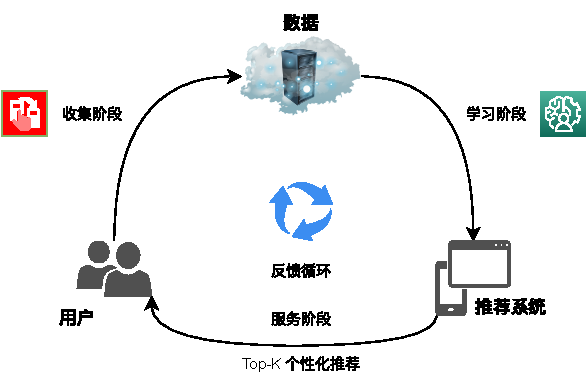
\includegraphics[width=.88\linewidth]{figure/rs-loops.drawio.pdf}
        \caption{推荐系统的反馈回路}
        \label{fig:rs-loop}
    \end{subfigure}
    \begin{subfigure}{0.49\linewidth}
        \centering
        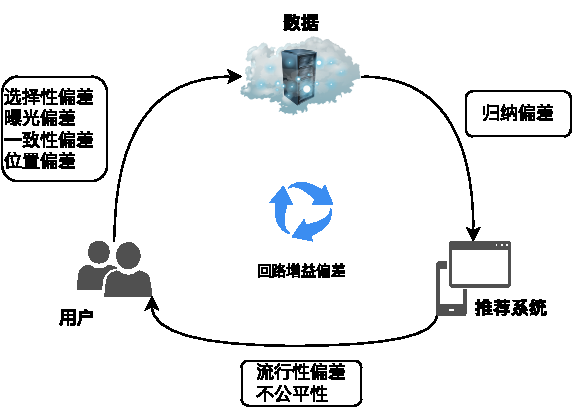
\includegraphics[width=.88\linewidth]{figure/rs-bias.drawio.pdf}
        \caption{反馈回路中的偏差}
        \label{fig:rs-bias}
    \end{subfigure}
    \caption{推荐系统中的反馈回路与偏差}
    \label{fig:rs-loop-bias}
\end{figure}

通常而言,推荐系统在收集、学习、服务三个阶段中通常存在八类偏差\cite{chen_bias_2021}。其中,与用户相关的偏差(bias in user)有选择性偏差(selection bias)、曝光偏差(exposure bias)、一致性偏差(conformity bias)、位置偏差(position bias);与数据有关的偏差(bias in data):流行性偏差(popularity bias)、不公平性(unfairness);与模型有关的偏差(bias in model)有归纳偏差(inductive bias);最后,在整个数据反馈回路中还存在回路增益偏差(bias amplification in loop)。本节将逐个介绍这些偏差。

(1)选择性偏差。选择性偏差通常出现在用户可以自由地为物品打分时。由于被系统采集到的打分并不能代替所有用户对该物品的打分,因此这里的打分数据通常是非随机性缺失(Missing Not at Random,MNAR)的。因此,系统可能会在数据中忽略某些用户的真实评价,进而导致推荐偏差;

(2)曝光偏差。曝光偏差通常出现在用户只能接触到一部分特定物品,而其余部分被默认的视为用户不喜欢的物品。这样的偏差可能导致用户错失一些可能符合其偏好的物品,进而降低了推荐系统的准确性;

(3)一致性偏差。一致性偏差通常出现在大多数用户倾向于与自己所属于的群体中其他人相似的行为,即使这样做违背了用户自己的偏好。这意味着反馈并不总是标志着用户的真实偏好。这种偏差可能导致用户无法得到真正符合自己需求的推荐结果;

(4)位置偏差。位置偏差通常发生在用户倾向于与推荐列表中位置靠前的物品进行交互,而不考虑物品实际的相关性。这可能导致一些物品始终处于推荐列表的前列,而其他物品则很难得到用户的关注;

(5)归纳偏差。归纳偏差是指模型在训练过程中,为了更好的被优化。引入某些假设,从而作出超越训练数据进行归纳。这种偏差可能导致模型出现过拟合,使得其在真实场景中的表现不佳;

(6)流行性偏差。流行性偏差是推荐系统中最常见的偏差之一,其具体含义是当某个物品被推荐的频率高于其受欢迎程度时,就会出现流行性偏差。这种偏差可能导致推荐系统的推荐结果过于倾向于那些已经广受欢迎的物品,而忽略了那些相对不太流行但仍然有一定用户喜好的物品,进而降低了系统的多样性;

(7)不公平性。不公平性是推荐系统中另一个重要的问题。这种偏差通常源于交互数据中的歧视行为,可能导致系统有意或无意地歧视某些个人或群体,并偏向于其他个人或群体。例如,一个基于性别的推荐系统可能会倾向于向女性用户推荐化妆品或服装,而向男性用户推荐电子产品或运动装备,从而对某些用户造成不公平的对待;

(8)回路增益偏差。回路增益偏差指出,推荐系统中的偏差在数据反馈回路中将被放大,从而进一步影响推荐结果。其中,与用户相关的偏差会影响用户未来的行为,导致数据中存在更多的偏差;与数据相关的偏差会放大数据的不平衡性,导致用户收到的推荐结果更加偏差。此外,模型中存在的偏差会对整个模型的学习产生系统性影响,进而在收集数据和推荐结果中引入更多的偏差。因此,应当采取措施来减少或消除这些偏差,以确保推荐结果的公平性和多样性。

\subsection{推荐系统的流行性偏差}
本文重点探讨推荐系统中流行性偏差现象的解决方法。在推荐系统中,长尾现象非常普遍:大部分用户会与少量热门物品进行交互。当模型在这种长尾数据上进行训练时,通常会高估受欢迎物品的分数,将不受欢迎的物品预测为负面。由于训练数据的分布不均,头部物品会更频繁地出现在训练数据中,对模型参数更新的贡献更大,从而导致严重的流行度偏差问题。因此,受欢迎的项目被推荐的频率甚至超过了它们在数据集中的真实受欢迎程度。忽视流行偏向会带来许多问题\cite{abdollahpouri_connection_2020}。1)流行偏向会降低个性化推荐的水平,削弱了推荐系统的多样性。由于不同用户的偏好是不同的,总是推荐受欢迎的项目会伤害用户体验,特别是那些喜欢小众项目的用户。2)流行偏向会降低推荐结果的公平性。流行的物品并不总是高质量的。过度推荐热门项目会降低其他项目的曝光率,即使它们是很好的匹配,这是不公平的。3)流行偏见会进一步增加流行物品的曝光机会,使得流行物品变得更加流行--这会导致未来训练数据变得更加不平衡,引发所谓的 "马太效应" 问题。

\section{基于图对比学习的标签感知推荐模型 TAGCL}
本节首先提出一种基于图对比学习的模型 TAGCL,该模型使用对比学习以克服数据中存在的流行度偏差,获得了优秀的推荐性能。

\subsection{模型架构}
TAGCL 延续使用了 LFGCF 结合用户-标签图与物品-标签图的设计,如图~\ref{fig:tagcal}。其中用户-标签图被用于捕获用户的偏好,而物品-标签图被用于获取物品的特质。在这种情况下,用户和项目并没有直接联系。虽然这可能有一些反直觉,但这有助于帮助简化图结构和训练过程。

\begin{figure}[!h]
    \centering
    \setlength{\belowcaptionskip}{-6mm}
    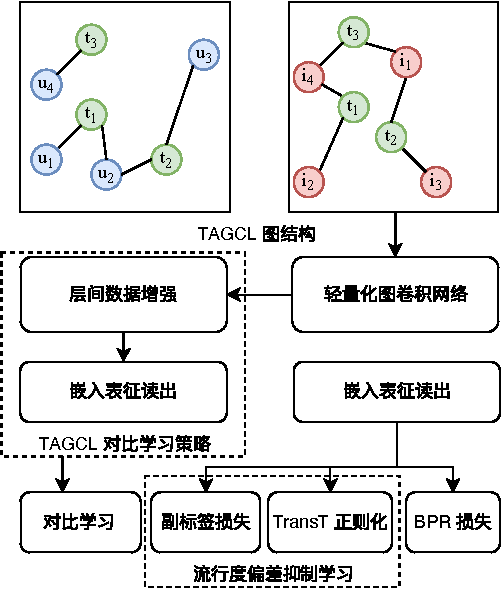
\includegraphics[width=.66\linewidth]{figure/tagcl.drawio.pdf}
    \caption{TAGCL 的模型架构}
    \label{fig:tagcal}
\end{figure}

与主流的推荐模型相似,每一个实体都被一个维度为 $d$ 的嵌入特征 (embedding) 描述。$e_u$ 和 $e_i$ 分别代表着用户和物品的嵌入表征,同时,与 LFGCF 不同,TAGCL 进一步区分了用户-标签图与物品-标签图所获得的标签嵌入特征, $e_{t(u)}$ ($e_{t(i)}$) 为用户-标签(物品-标签)图所获得的嵌入表征。

\subsection{嵌入表征的数据增强}
近年来,由于对比学习在计算机视觉和自然语言处理任务中表现出从大量无标签数据中提取有效特征的潜力,引起了广泛的研究兴趣\cite{chen_simclr_2020,gidaris_unsupervised_2018,devlin_bert_2019,gao_simcse_2021}。对比学习在推荐系统中的应用需要两个关键组件:数据增强和对比学习任务。本节主要关注如何有效地进行数据增强以创建差异最大化的对比视图。目前有两种主流的图数据增强,Wang 等人\cite{wu_self-supervised_2021}提出了推荐模型 SGL,图结构使用边丢弃、节点丢弃、随机游走等进行变换,来创建不同的子图。Yu 等人\cite{yu_simgcl_2022}提出了推荐模型 SimGCL,对嵌入表征加入随机噪声,从而创建不同的视图。实验证明,SimGCL 添扰动的方式更为简单有效。受到 SimGCL 设计的启发,TAGCL 中数据增强是通过对嵌入表征添加小的扰动来进行的。与应用各种操作修改图结构相比,对嵌入表征进行轻微扰动为每个节点创造了相似的视图。通过增加小的扰动,TAGCL 实现了更好的性能,并提高训练效率。以用户 $u$ 的嵌入表征为例。嵌入表征的数据增强可以被定义为:
\begin{equation}
    e_u' = e_u + \epsilon \delta_u' \quad e_u'' = e_u + \epsilon \delta_u'' 
\end{equation}
其中,扰动 $\delta'/\delta''$ 是服从正态分布的归一化噪声,$\epsilon$ 则控制扰动的强度。最终,噪声使用 SoftMax 函数进行归一化。

\subsection{多任务学习框架}
TAGCL 采用了多任务学习的方式,主要包括推荐任务、对比学习任务和和流行度抑制学习任务。本文采用了 BPR 作为优化函数。BPR 损失函数通过预测更高的分数来记录交互记录,对于个性化排名推荐特别有效。其数学表达式为:
\begin{equation}
    \mathcal{L}_{rec} = -\sum_{u \in \mathcal{U}}\sum_{i \in \mathcal{N}_u}\sum_{i' \notin \mathcal{N}_u} ln \sigma (\hat{y}_{ui} - \hat{y}_{ui'}) + \lambda||\Theta||^2
\end{equation}
其中,$\lambda$ 控制着 $L_2$ 正则函数的强度。下文将阐述其余学习任务损失函数的概念和设计。

\subsubsection{对比学习任务}
经过数据增强后,每个节点在图中被构建为两种视图。对比学习的任务就是最大化提高同一节点视图的一致性。对比学习损失函数通过调节 SoftMax 函数中的温度参数$\tau$,可以对数据中的长尾标签进行不同程度的挖掘。最终,我们使用 InfoNCE \cite{oord_rl4cp_2018} 作为对比学习损失函数,以用户-标签图为例可以被表征为:
\begin{equation}
    \begin{aligned}
        \mathcal{L}_{cl}^{user} &= \sum_{u \in \mathcal{U}} -ln{\frac{exp(e_u'^T e_u''/\tau)}{\sum_{v \in \mathcal{U}}exp(e_u'^T e_{v}''/\tau)}} \quad u \neq v  \\
        \mathcal{L}_{cl}^{tag(u)} &= \sum_{t \in \mathcal{T}} -ln{\frac{exp(e_{t(u)}'^T e_{t(u)}''/\tau)}{\sum_{s \in \mathcal{T}}exp(e_{t(u)}'^T e_{s(u)}''/\tau)}} \quad t \neq s  \\
        \mathcal{L}_{cl}^{\mathcal{G}_{UT}} &= \mathcal{L}_{cl}^{user} + \mathcal{L}_{cl}^{tag(u)} 
        \label{infonce}
    \end{aligned}
\end{equation}
其中的超参数 $\tau$ 为SoftMax中的温度系数。类似的,在物品-标签图也使用了类似的对比学习损失函数 $\mathcal{L}_{cl}^{\mathcal{G}_{IT}}$。因此,TAGCL 的完整对比学习损失函数被定义为:
\begin{equation}
    \begin{aligned}
        \mathcal{L}_{cl} = \mathcal{L}_{cl}^{\mathcal{G}_{UT}} + \mathcal{L}_{cl}^{\mathcal{G}_{IT}}
    \end{aligned}
\end{equation}

\subsubsection{流行度偏差抑制学习任务}
为了平衡性能和推荐系统的公平性,本文提出了两个目标函数:负标签损失和TransT正则化。在训练过程中,每条社会标注数据都是形如 $<u, t, i> \in \mathcal{A}$ 的三元组。由于推荐系统中只有很少量的正向互动,因此通常需要从未发生交互的样本中随机采样一部分用于模型训练。在 TAGCL 中,我们将物品采样进一步扩展到标签中,因此训练集 $\mathcal{D}$ 可以扩展为五元组 $(u, t, t', i, i')$。
\begin{equation}
    \mathcal{D} = \{(u, t, t', i, i')|(u, t, i) \in \mathcal{A} \cap (u, t',i) \notin \mathcal{A} \cap (u, t,i') \notin \mathcal{A} \} 
\end{equation}

为了在标签领域进行采样,本文首先从那些没有被任何用户分配的标签中进行采样。受到标签与物品之间交互分布差异的启发,提出了负标签损失作为一种优化推荐系统公平性的损失。对于一个五元组$(u, t, t', i, i')$,负标签损失函数定义为:
\begin{equation}
    \mathcal{L}_{nt} = -\sum_{(u, t, t', i, i')\in \mathcal{D}}ln[\sigma(e_{t(i)}^T e_i - e_{t'(i')}^T e_{i'})] 
\end{equation}
其中$\sigma$是激活函数。由于标签的选择集中于少数标签,因此标签和物品之间的关系相对不受数据偏差的影响。因此,负标签损失将物品和标签的嵌入向量的内积作为输入,最大化正配对和负配对之间的乘积差。更高的内积值意味着标签-物品对之间的相关性更高。

本节进一步提出了一种新的 TransT 正则化函数,旨在以一种公平的方式推进推荐系统。由于负标签损失只考虑物品-标签图 ${\mathcal{G}_{IT}}$ 中标签的嵌入表征 $e_{t(i)}$,而摒弃了用户-标签图 ${mathcal{G}_{IT}}$ 中的嵌入表征。不同于 TransTag\cite{chen_tgcn_2020} 和 LFGCF 中提出的 TransRT。本节将 $\mathcal{G}_{UT}$ 和 $\mathcal{G}_{IT}$ 之间,标签嵌入的差异(即$e_{t(u)} - e_{t(i)}$),视为沟通用户和物品之间的桥梁。具体来说,在记录 $(u, t, i) \in \mathcal{A}$ 的情况下,物品 $i$ 的嵌入表征 $e_i$ 应该接近于 $e_u + e_{t(u)} - e_{t(i)}$。由于大多数数据遵循长尾分布,当物品 $i$ 受欢迎时,$e_u$ 会朝着 $e_i$ 的方向更新。同时,$e_u$ 和 $e_i$ 是在信息聚合过程中从标签嵌入中聚合出来的,这使得它们局部相似。虽然将 $e_t$ 假定为实体间关系的嵌入与我们的直觉一致,即标签是连接用户和项目的桥梁,但当标签在社会标注图结构中与用户和项目具有相同的重要性时,这种方法并不实际。本文的独特设计 $e_{t(u)} - e_{t(i)}$ 可以充分利用 $e_t$,并揭示出用户和物品之间的实质性关系。最终,TransT 正则化函数可以定义为:
\begin{equation}
    \mathcal{L}_{T} = \sum_{(u, t, i) \in \mathcal{A}}||e_u + (e_{t(u)} - e_{t(i)}) - e_i||_2
\end{equation}

\subsection{优化目标函数}
综合本节提出的 BPR推荐损失、负标签损失、对比学习损失和 TransT 正则化函数被整合成 TAGCL 的最终的优化目标函数:
\begin{equation}
    \mathcal{L} = \mathcal{L}_{rec} + \alpha \mathcal{L}_{cl} + \beta \mathcal{L}_{nt} + \gamma \mathcal{L}_{T}
    \label{loss}
\end{equation}
其中,$\alpha$, $\beta$ 和 $\gamma$ 分别控制着每一个损失函数的强度。由于 TAGCL 仅有第 0 层的嵌入表征为可训练参数,即 $\Theta = \{e_u^{(0)}, e_{t(u)}^{(0)}, e_{t(i)}^{(0)}, e_i^{(0)}\}$。最后模型使用 Adam 优化,并在小批量策略进行。本文使用早停策略来防止模型被过度训练。
\section{本章小结}
本章主要介绍了对比学习及其在推荐系统中的应用。对比学习是一种有效的难例挖掘方法,可以克服推荐数据中存在的流行度偏差。本章将对比学习引入到推荐系统中,并由 NCE 损失函数推导出 InfoNCE 损失函数。相比于传统的 NCE 损失函数,InfoNCE 损失函数能够更好地捕捉物品间的互信息,提升了推荐系统的性能。 在本章的研究中,本文提出了一种新的模型设计架构 TAGCL。TAGCL 模型采用了多任务学习的框架,通过同时学习多个任务,提高了模型的泛化能力。该模型采用了深度神经网络的思想,并采用了类似于 TransE 的则化函数 TransT,以促进推荐系统的公平性。